
\begin{frame}
 \begin{center}
  \Huge Statistics of Interest
 \end{center}

\end{frame}

\begin{frame}{Sense Prior}
\begin{itemize}

\item \textbf{Sense Prior} The number of times a particular ``sense'' of an entity is used \medskip
\item There are several ``Gingerbreads'' (Android 2.3, The novel) \medskip
\item Sense prior would tell us how frequent is \emph{Gingerbread the OS} compared with \emph{Gingerbread the novel}  \medskip
\item $Sense Prior(Si , E) = P (\text{E appears as the ith sense}) = P (Si |E) $ \medskip
\item Different from mention prior! (Number of times a mention links to a particular entity)
\end{itemize}
\end{frame}

\begin{frame}{Sense Prior}{Example (Hypothetical)}
  \begin{textblock*}{120pt}[.50,.5](70pt,70pt)
  \begin{figure}[h]
 
 
\includegraphics[bb=0 0 200 150, scale=0.4]{./baske.jpg}
 
 % baske.jpg: 200x150 pixel, 72dpi, 7.06x5.29 cm, bb=0 0 200 150
\end{figure}
   \centering 
   Basketballer (60\%)
\end{textblock*}
  \begin{textblock*}{120pt}[.50,.5](280pt,80pt)
  \begin{figure}[h]
 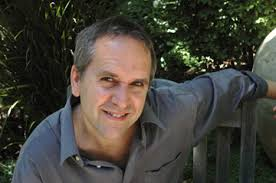
\includegraphics[bb=0 0 200 150, scale=0.4]{./prof.jpg}
 % baske.jpg: 200x150 pixel, 72dpi, 7.06x5.29 cm, bb=0 0 200 150
\end{figure}
\centering
   Professor (30\%)
\end{textblock*}
  \begin{textblock*}{120pt}[.50,.5](70pt,200pt)
  \begin{figure}[h]
 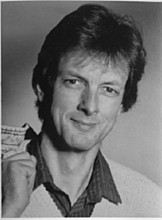
\includegraphics[bb=0 0 200 150, scale=0.4]{./botanist.jpg}
 % baske.jpg: 200x150 pixel, 72dpi, 7.06x5.29 cm, bb=0 0 200 150
\end{figure}
\centering
Botanist (8\%)
\end{textblock*}
  \begin{textblock*}{120pt}[.50,.5](260pt,200pt)
  \begin{figure}[h]
 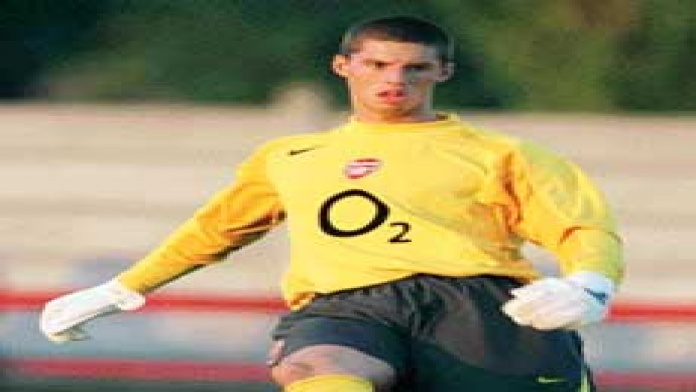
\includegraphics[bb=0 0 200 150, scale=0.16]{./footballer.jpg}
 % baske.jpg: 200x150 pixel, 72dpi, 7.06x5.29 cm, bb=0 0 200 150
\end{figure}
\centering
Footballer (2\%)
\end{textblock*}
  \begin{textblock*}{120pt}[.50,.5](200pt,140pt)

\large{Michael Jordan}

\end{textblock*}

\end{frame}


\begin{frame}{Entity Bigrams}{Motivation}
 \begin{figure}[h]
 \centering
 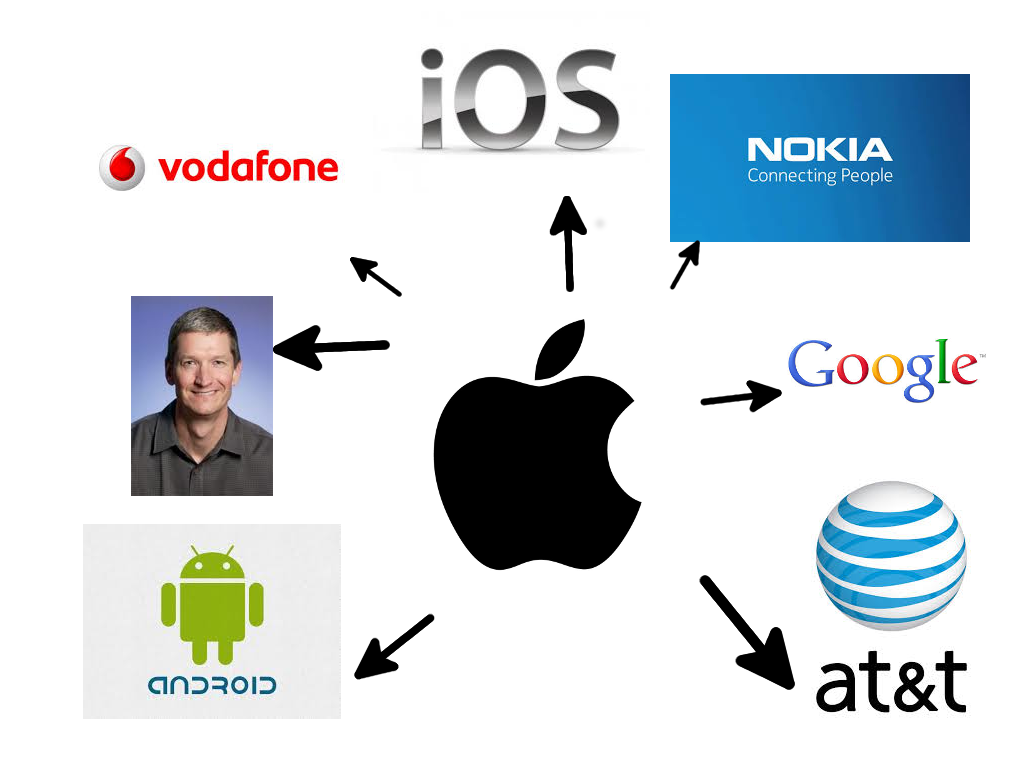
\includegraphics[bb=0 0 1024 768, scale=0.25]{./entitycoocc.png}
 % entitycoocc.png: 1024x768 pixel, 72dpi, 36.12x27.09 cm, bb=0 0 1024 768
 \caption{Entities Frequently Appear with related entities}
\end{figure}

\end{frame}

\begin{frame}{Entity Bigrams}
\begin{itemize}
 \item \textbf{Entity Bigrams} Counts the number of times two given entities, taking two given senses appear together. \medskip
\item Eg. : Number of times Nokia \url{http://en.wikipedia.org/wiki/Nokia} appears with Gingerbread \url{http://en.wikipedia.org/wiki/Gingerbread_(operating_system)} \medskip


 \item $\text{Entity Bi Gram}(E2|E1) = P (E2\ follows\ E1) = P (E2|E1)$
 \end{itemize}
\end{frame}


\begin{frame}{Entity Bigrams}{Application : Finding Closely Related Entities}
 \begin{figure}[h]
 \centering
 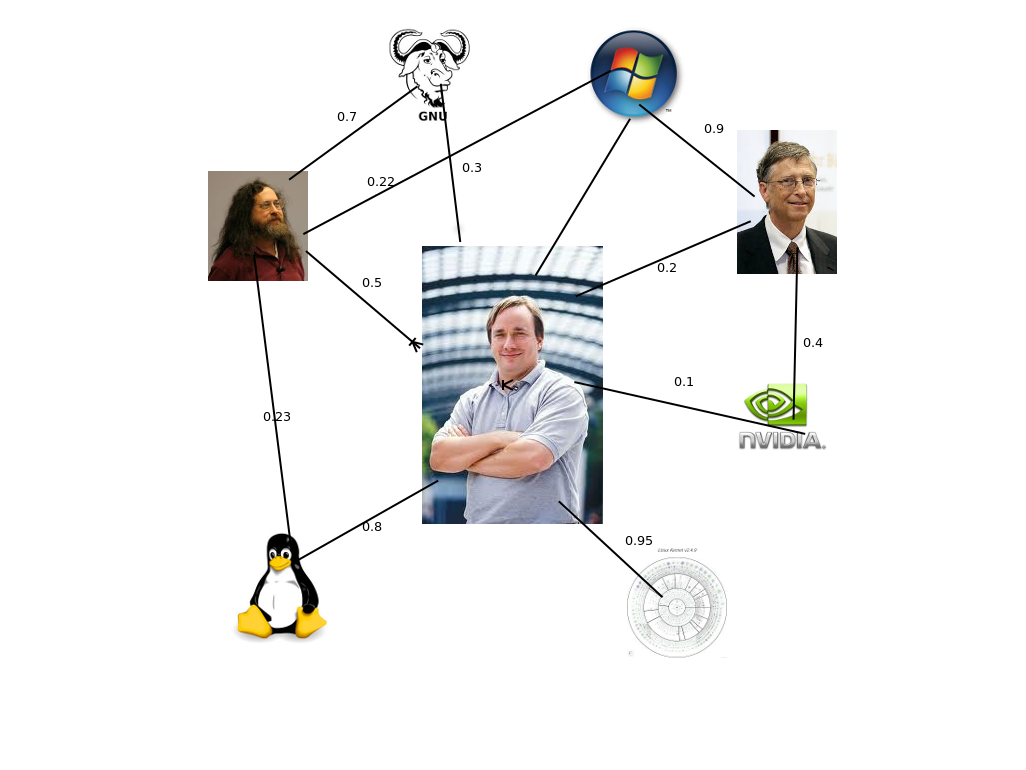
\includegraphics[bb=0 0 1024 768, scale=0.30]{./rel.png}
 % entitycoocc.png: 1024x768 pixel, 72dpi, 36.12x27.09 cm, bb=0 0 1024 768
 \caption{Starting from the central entity, apply personalized page rank}
\end{figure}

\end{frame}
